
%%%%%%%%%%%%%%%%%%%%%%%%%%%%%%%%%%%%%%%%%%%%%%%%%%%%%%%%%%
%%
%% This is the "PREAMBLE". Here we define the type of document and load in any packages we might want. You can also set parameters %% % and create your own short-hand here.
%%
%%%%%%%%%%%%%%%%%%%%%%%%%%%%%%%%%%%%%%%%%%%%%%%%%%%%%%%%%%

 \documentclass[9pt]{article}
 
 \def\solutions{1}


 \usepackage{amsmath}
 \usepackage{amssymb}
 \usepackage{graphicx}    % needed for including graphics e.g. EPS, PS \usepackage{tikz}
 \usepackage{tikz}\usetikzlibrary{calc,arrows.meta,quotes}
 \usepackage{tikzsymbols}
 \usepackage{relsize}
 \usepackage{forest}
 \usetikzlibrary{patterns,decorations.pathreplacing,shapes,arrows}
 \usepackage{algorithm2e}
 \topmargin -2.5cm        % read Lamport p.163
 \oddsidemargin -0.04cm   % read Lamport p.163
 \evensidemargin -0.04cm  % same as oddsidemargin but for left-hand pages
 \textwidth 16.59cm
 \textheight 25.94cm
% \pagestyle{empty}        % Uncomment if don't want page numbers
 \pagenumbering{gobble}
 \parskip 7.2pt           % sets spacing between paragraphs
 %\renewcommand{\baselinestretch}{1.5} 	% Uncomment for 1.5 spacing between lines
 \parindent 0pt		  % sets leading space for paragraphs

% No date in header
\date{}

\usepackage{hyperref}
\hypersetup{
    colorlinks=true,
    linkcolor=blue,
    filecolor=magenta,      
    urlcolor=cyan,
}
\usepackage{amsthm}
\usepackage{fancyhdr}
\pagestyle{fancy}
\setlength{\headsep}{36pt}

\usepackage{hyperref}
\graphicspath{ {./images/} }

\newcommand{\lp}{\left(}
\newcommand{\rp}{\right)}
\newcommand{\lb}{\left[}
\newcommand{\rb}{\right]}
\newcommand{\ls}{\left\{}
\newcommand{\rs}{\right\}}
\newcommand{\lbar}{\left|}
\newcommand{\rbar}{\right|}
\newcommand{\ld}{\left.}
\newcommand{\rd}{\right.}

\newcommand{\myexists}{\exists \hspace{.3mm}}

\newcommand{\hs}{\hspace{.75mm}}
\newcommand{\bs}{\hspace{-.75mm}}
\newcommand{\nin}{\noindent}

\newcommand{\fx}{f\bs\left( x \right)}
\newcommand{\gx}{g\bs\left( x \right)}
\newcommand{\qx}{q\bs\left( x \right)}

\newcommand{\nn}{\nonumber}

\newcommand{\vfive}{\vspace{5mm}}
\newcommand{\vthree}{\vspace{3mm}}

\newcommand{\fof}[1]{f\lp #1\rp}
\newcommand{\gof}[1]{g\lp #1\rp}
\newcommand{\qof}[1]{q\lp #1\rp}

\newcommand{\myp}[1]{\left( #1 \right)}
\newcommand{\myb}[1]{\left[ #1 \right]}
\newcommand{\mys}[1]{\left\{ #1 \right\}}
\newcommand{\myab}[1]{\left| #1 \right|}

\newcommand{\myj}{_j}
\newcommand{\myjp}{_{j+1}}
\newcommand{\myjm}{_{j-1}}

\newcommand{\f}[1]{f\hspace{-1mm}\left( #1 \right)}
\newcommand{\fp}[1]{f'\hspace{-1mm}\left( #1 \right)}
\newcommand{\g}[1]{g\hspace{-1mm}\left( #1 \right)}
\newcommand{\gp}[1]{g'\hspace{-1mm}\left( #1 \right)}
\newcommand{\q}[1]{q\hspace{-1mm}\left( #1 \right)}
\newcommand{\qp}[1]{q'\hspace{-1mm}\left( #1 \right)}
\newcommand{\Px}[1]{P\hspace{-1mm}\left( x_{#1} \right)}
\newcommand{\Qx}[1]{Q\hspace{-1mm}\left( x_{#1} \right)}

\newcommand{\tten}[1]{\times 10^{#1}}

\newcommand{\aij}[1]{a_{#1}}
\newcommand{\bij}[1]{b_{#1}}
\newcommand{\rij}[1]{r_{#1}}

\newcommand{\R}[1]{\mathbb{R}^{#1}}

\newcommand{\ith}{i^{\textrm{th}}}
\newcommand{\jth}{i^{\textrm{th}}}
\newcommand{\kth}{i^{\textrm{th}}}

\newcommand{\inv}[1]{{#1}^{-1}}

\newcommand{\bx}{\mathbf{x}}
\newcommand{\bv}{\mathbf{v}}
\newcommand{\bw}{\mathbf{w}}
\newcommand{\by}{\mathbf{y}}
\newcommand{\bb}{\mathbf{b}}
\newcommand{\be}{\mathbf{e}}
\newcommand{\br}{\mathbf{r}}
\newcommand{\xhat}{\hat{\mathbf{x}}}

\newcommand{\beq}{\begin{eqnarray}}
\newcommand{\eeq}{\end{eqnarray}}

\newcommand{\ben}{\begin{enumerate}}
\newcommand{\een}{\end{enumerate}}

\newcommand{\bsq}{\mathsmaller{\blacksquare}}

\newcommand{\iter}[1]{^{\myp{#1}}}

% matrix macro
\newcommand{\mymat}[1]{
\left[
\begin{array}{rrrrrrrrrrrrrrrrrrrrrrrrrrrrrrrrrrrrrrr}
#1
\end{array}
\right]
}

\newcommand{\makenonemptybox}[2]{%
%\par\nobreak\vspace{\ht\strutbox}\noindent
\item[]
\fbox{% added -2\fboxrule to specified width to avoid overfull hboxes
% and removed the -2\fboxsep from height specification (image not updated)
% because in MWE 2cm is should be height of contents excluding sep and frame
\parbox[c][#1][t]{\dimexpr\linewidth-2\fboxsep-2\fboxrule}{
  \hrule width \hsize height 0pt
  #2
 }%
}%
\par\vspace{\ht\strutbox}
}
\makeatother

\newcommand{\smallaug}[1]{
\left[
\begin{array}{rr|r}
#1
\end{array}
\right]
}

%%%%%%%%%%%%%%%%%%%%%%%%%%%%%%%%%%%%%%%%%%%%%%%%%%%%%%%%%%
%%
%% End of PREAMBLE
%%
%%%%%%%%%%%%%%%%%%%%%%%%%%%%%%%%%%%%%%%%%%%%%%%%%%%%%%%%%%



% ======================================================================================
% Actual document starts here. 
% PLEASE FILL IN YOUR NAME AND STUDENT ID.
% ======================================================================================
\begin{document}

\lhead{{\bf CSCI 3104, Algorithms \\ Problem Set 6 (50 points)} }
\rhead{Name: \fbox{Felipe Lima} \\ ID: \fbox{109290055} \\ {\bf Due March 5, 2021 \\ Spring 2021, CU-Boulder}}
\renewcommand{\headrulewidth}{0.5pt}

\phantom{Test}

\begin{small}
\textit{Advice 1}:\ For every problem in this class, you must justify your answer:\ show how you arrived at it and why it is correct. If there are assumptions you need to make along the way, state those clearly.
\vspace{-3mm} 

\textit{Advice 2}:\ Verbal reasoning is typically insufficient for full credit. Instead, write a logical argument, in the style of a mathematical proof.\\
\vspace{-3mm} 

\textbf{Instructions for submitting your solution}:
\vspace{-5mm} 

\begin{itemize}
	\item The solutions \textbf{should be typed} and we cannot accept hand-written solutions. \href{http://ece.uprm.edu/~caceros/latex/introduction.pdf}{Here's a short intro to Latex.}
	\item You should submit your work through \href{https://www.gradescope.com/courses/218966}{\textbf{Gradescope}} only.
	\item The easiest way to access Gradescope is through our Canvas page. There is a Gradescope button in the left menu.
	\item Gradescope will only accept \textbf{.pdf} files.
	\item \href{https://www.youtube.com/watch?v=u-pK4GzpId0&feature=emb_logo}{It is vital that you match each problem part with your work.} Skip to 1:40 to just see the matching info.
\end{itemize}
\vspace{-4mm} 
\end{small}

\hrulefill
\pagebreak



\ben
%%%%%%%%%%%%%%%%%%%%%%%%%%%%%%%%%%%%%%%%%%%%%%%%%%%%%%%%
% PROBLEM  ONE %% PROBLEM  ONE %% PROBLEM  ONE %% PROBLEM  ONE %% PROBLEM  ONE %
%==============================================================================
% Problem 1: Greedy Algorithms
%==============================================================================
% PROBLEM  ONE %% PROBLEM  ONE %% PROBLEM  ONE %% PROBLEM  ONE %% PROBLEM  ONE %
%%%%%%%%%%%%%%%%%%%%%%%%%%%%%%%%%%%%%%%%%%%%%%%%%%%%%%%%

\item 

\begin{enumerate}

\item Consider designing an algorithm for issuing coins from a vending machine. This algorithm should take in an amount of change needed $x$ and issues the minimum number of coins whose value sums to $x$. Given an ordered set of coin denominations, $C = \{c_{1}, c_{2}, ... \}$, a typical greedy approach is to choose the largest coin $c_k$ such that $c_k \leq x$, then set $x = x - c_k$ and recurse. Using the set $C = \{1, 5, 10, 25\}$, list the coins returned for the given values of $x$.

\textit{Example} $x = 24$. \textit{Solution:} [10, 10, 1, 1, 1, 1]

\begin{enumerate}
    \item $x = 16$
    \item $x = 49$
    \item $x = 31$
\end{enumerate}

\item Provide a set $C$ of coin denominations for which the greedy approach given in (a) is \textbf{not} always optimal. Give an example value of $x$ for which the greedy solution and optimal solution differ, and show that these two solutions differ by listing the coins the greedy solution would pick versus the optimal set of coins.

\item Suppose you are late for (an in-person!) class and are trying to cram important items from your apartment into your backpack to take to campus. However, your backpack only has $k$ total space and you have a variety of items $I = \{i_{1}, i_{2}, ... \}$, each of which has a value $v(i)$ and size $s(i)$. We want to choose the set of items $I^*$ that maximizes the sum of values $\sum_{i \in I^*} v(i)$ while still fitting in the backpack: $\sum_{i \in I^*} s(i) \leq k$. 

One greedy approach to the problem is to take the item $i_{n}$ with max $v(i_n)$ such that $s(i_{n}) \leq k$, then set $k = k - s(i_n)$, remove $i_n$ from $I$ and recurse. Given the following set of items, and with a backpack size of $k = 20$, provide the optimal and greedy solutions and note whether or not they differ.

\begin{center}
\begin{tabular}{c|c|c}
Item Name & Value & Size \\ \hline
Laptop & 20 & 12 \\ 
Phone Charger & 13 & 8 \\
Notebook & 18 & 11 \\
Pencil & 3 & 2 \\
Textbook & 22 & 15
\end{tabular}
\end{center}

\item Another greedy approach to this problem is to first calculate each item's value \textit{density}, defined as $d(i) = \frac{v(i)}{s(i)}$, then choose items in order of max $d(i)$ until the backpack is full. More specifically, this approach chooses the item $i_n$ with max $d(i_n)$ such that $s(i_n) \leq k$, then sets $k = k - s(i_n)$, removes $i_n$ from $I$, and recurses. Given the same set of items above, this time with a backpack size of $k = 21$, provide the optimal solution and this greedy solution and note whether or not they differ.

\end{enumerate}

  \if\solutions1
  \vspace{2mm}
  
  \textbf{Solution:}   \\
%==============================================================================
% STUDENTS: TYPE YOUR SOLUTIONS HERE. (Between \textbf{Solution:} and \fi )
%==============================================================================
\begin{enumerate}

    \item 
    \begin{enumerate}
        \item  $x = 16$. \textit{Solution:} $[10,5,1]$
        \item  $x = 49$. \textit{Solution:} $[25,10,10,1,1,1,1]$
        \item  $x = 31$. \textit{Solution:} $[25,5,1]$
    \end{enumerate}
    
    \item
        Let a set $C = {10,50,70}$\\
        Let $x=100$\\
        The greedy solution will be: $[70,10,10,10]$\\
        The optimal solution will be: $[50,50]$\\
        On the optimal solution we only use 2 coins while the greedy solution we use 4 coins. Thus they differ and the greedy algorithm is not optimal.
    
    
    \fi
    
    \newpage
    \vspace{5mm}
    \item 
        The greedy algorithm would choose the Textbook with $Value = 22$ and $Size = 15$ and the pencil with $Value = 3$ and $Size = 2$, leaving $k=3$ space left.\\\\
        The optimal solution would choose so the value is maximized while fitting the most objects. To do so, it would pick the Laptop $Value = 20$ and $Size = 12$ and the Phone Charger $Value = 13$ and $Size = 8$.\\\\
        The optimal and the greedy solution differ in the choice of objects but are the same in the number of objects picked. The optimal solution ends up with a value of $33$ while the greedy solution ends up with value of $25$.
    
    \item \phantom{.}
    \begin{center}
    \begin{tabular}{c|c|c|c}
    Item Name & Value & Size & Density\\ \hline
    Laptop & 20 & 12 & 1.667\\ 
    Phone Charger & 13 & 8 & 1.625 \\
    Notebook & 18 & 11 & 1.636\\
    Pencil & 3 & 2 & 1.5 \\
    Textbook & 22 & 15 & 1.467
    \end{tabular}
    \end{center}
        The greedy algorithm would choose the Laptop with $Density = 1.667$ and $Size = 12$ and the phone charger with $Density = 1.625$ and $Size = 8$. Totalizing $Value = 33$ and $Size = 20$ while leaving $k=1$ space left.\\\\
        The optimal solution would try instead to end up with $k=0$. Therefore it would pick the phone charger $Density = 1.625$ and $Size = 8$, the pencil $Density = 1.5$ and $Size = 2$, and the notebook $Density = 1.636$ and $Size = 11$. Totalizing $Value = 34$ and $Size = 21$.\\\\
        In this situation the optimal solution differ by picking one more object than the greedy solution and totaling a bigger value. 
    \end{enumerate}

\newpage


%%%%%%%%%%%%%%%%%%%%%%%%%%%%%%%%%%%%%%%%%%%%%%%%%%%%%%%%
% PROBLEM TWO %% PROBLEM TWO %% PROBLEM TWO %% PROBLEM TWO %% PROBLEM TWO %
%==============================================================================
% Problem 2: Interval Scheduling
%==============================================================================
% PROBLEM TWO %% PROBLEM TWO %% PROBLEM TWO %% PROBLEM TWO %% PROBLEM TWO %
%%%%%%%%%%%%%%%%%%%%%%%%%%%%%%%%%%%%%%%%%%%%%%%%%%%%%%%%

\vspace{5mm}

\item Suppose we have a number of events $m_{i}$. Each event starts at time $s_{i}$ and finishes at time $e_{i}$, where $0 \leq s_{i} < e_{i}$. We represent the event $m_{i}$ with the closed interval $[s_{i}, e_{i}].$ Our goal is to construct a maximum size set of events, where no two events in the set overlap (note that two events $m_{i}$ and $m_{j}$ where $m_{i} = [\cdot, x]$ and $m_{j} = [x, \cdot]$ are not considered to overlap). \\

Suppose the following intervals are provided.

\begin{center}
\begin{tabular}{c|c}
Event Index & Interval \\ \hline
A & $[1, 4]$ \\ 
B & $[2, 3]$ \\
C & $[3, 6]$ \\
D & $[5, 9]$ \\
E & $[7, 11]$
\end{tabular}
\end{center}

\begin{enumerate}

\item Give the optimal set of events for this example set of intervals.

\item Consider the following greedy approach: at each step, select the event with the earliest starting time that does not conflict with any event already in our set. Show that this approach is not optimal by providing the greedy solution generated by this approach for the above example intervals.

\item Consider a second greedy approach: first order the events by length. Then, at each step, select the event with the shortest length that does not conflict with any event already in our set. While this approach generates the optimal set for the above example, it is not guaranteed to do so for this problem generally. Give a set of 5 intervals for which this second greedy approach fails to generate the optimal solution. Explicitly state both the optimal solution and the solution generated by this approach for your example.

\item State a greedy approach to this problem that always finds the optimal solution.

\end{enumerate}

\if\solutions1
\vspace{2mm}

\textbf{Solution:} \\
%==============================================================================
% STUDENTS: TYPE YOUR SOLUTIONS HERE. (Between \textbf{Solution:} and \fi )
%==============================================================================

\begin{enumerate}
    \item 
        Let $S$ be the optimal set of events\\
        $S=[B,C,E]$
    \item
        The greedy approach selecting events by the earliest starting time will result in the following set:\\
        $G=[A,D]$\\
        Therefore, the greedy algorithm is not optimal. Set $S$ (from question a) resulted in more events than set $G$.
    \item \phantom{.}
        \begin{center}
        \begin{tabular}{c|c}
        Event Index & Interval \\ \hline
        A & [1,3] \\ 
        B & [3,5] \\
        C & [5,7] \\
        D & [7,9] \\
        E & [4.5,5.5]\\
        \end{tabular}
        \end{center}
        Order events by shortest length:\\
        $$E,A,B,C,D$$\\
        The greedy solution would be: $[E,A,D]$\\
        The optimal solution would be: $[A,B,C,D]$
    \item
        Greedy approach to this problem that always finds the optimal solution: At each step select the elements with the earliest starting time that does not conflict with any events already in our set.
\end{enumerate}


\fi
\newpage


%%%%%%%%%%%%%%%%%%%%%%%%%%%%%%%%%%%%%%%%%%%%%%%%%%%%%%%%
% PROBLEM THREE %% PROBLEM THREE %% PROBLEM THREE %% PROBLEM THREE %% PROBLEM THREE %
%==============================================================================
% Problem 3: Huffman Encoding
%==============================================================================
% PROBLEM THREE %% PROBLEM THREE %% PROBLEM THREE %% PROBLEM THREE %% PROBLEM THREE %
%%%%%%%%%%%%%%%%%%%%%%%%%%%%%%%%%%%%%%%%%%%%%%%%%%%%%%%%

\vspace{5mm}

\item The following problems deal with the concept of Huffman Coding.

\begin{enumerate}

\item Suppose your friend tells you that they have written a program to generate Huffman codes. You test it out by entering the text of \textit{Wuthering Heights}, and it generates the following codes for the first several letters of the alphabet:

\begin{center}
\begin{tabular}{c|c}
Letter & Code \\ \hline
a & 01 \\ 
b & 00101 \\
c & 101 \\
d & 00111 \\
e & 1 \\
f & 000 \\
g & 0011 \\
... & ...
\end{tabular}
\end{center}

Even without knowing the exact distribution of letters in \textit{Wuthering Heights}, you are immediately suspicious of your friend's program. Explain why this is not a possible valid set of Huffman codes.

\item Generate Huffman codes for the following set of letters with their given frequencies. Show your work by writing out the list of nodes and their respective frequencies available at each step. You can refer to nodes containing multiple letters in their subtree using a capitalized list of letters in alphabetical order; for example, if after some step you had a node representing a subtree containing \textit{a} and \textit{e} with frequency 0.6, you could refer to it in your list as $(AE, 0.6)$. Don't forget to list the final codes at the end!

\begin{center}
\begin{tabular}{c|c}
Letter & Frequency \\ \hline
a & 0.25 \\ 
b & 0.15 \\
c & 0.2 \\
d & 0.05 \\
e & 0.35
\end{tabular}
\end{center}


\end{enumerate}

\if\solutions1
\vspace{2mm}

\textbf{Solution:} \\
%==============================================================================
% STUDENTS: TYPE YOUR SOLUTIONS HERE. (Between \textbf{Solution:} and \fi )
%==============================================================================

\begin{enumerate}
    \item
        This Huffman code is not valid because it does not follow the prefix property. In the given case, the code 101 could be the letter $c$ or the letter $e$ followed by the letter $a$.    
    \item
        Construct a tree by connecting the smallest two frequencies with a common root.
        $$d:0.05 \phantom{......} b:0.15 \phantom{......} c:0.2 \phantom{......} a:0.25 \phantom{......} e:0.35$$ \\\\
    % You can use the template below for listing your codes
    \begin{center}
    \begin{tabular}{c|c}
    Letter & Code \\ \hline
    a & 10 \\ 
    b & 001 \\
    c & 01 \\
    d & 000 \\
    e & 11
    \end{tabular}
    \end{center}
\newpage
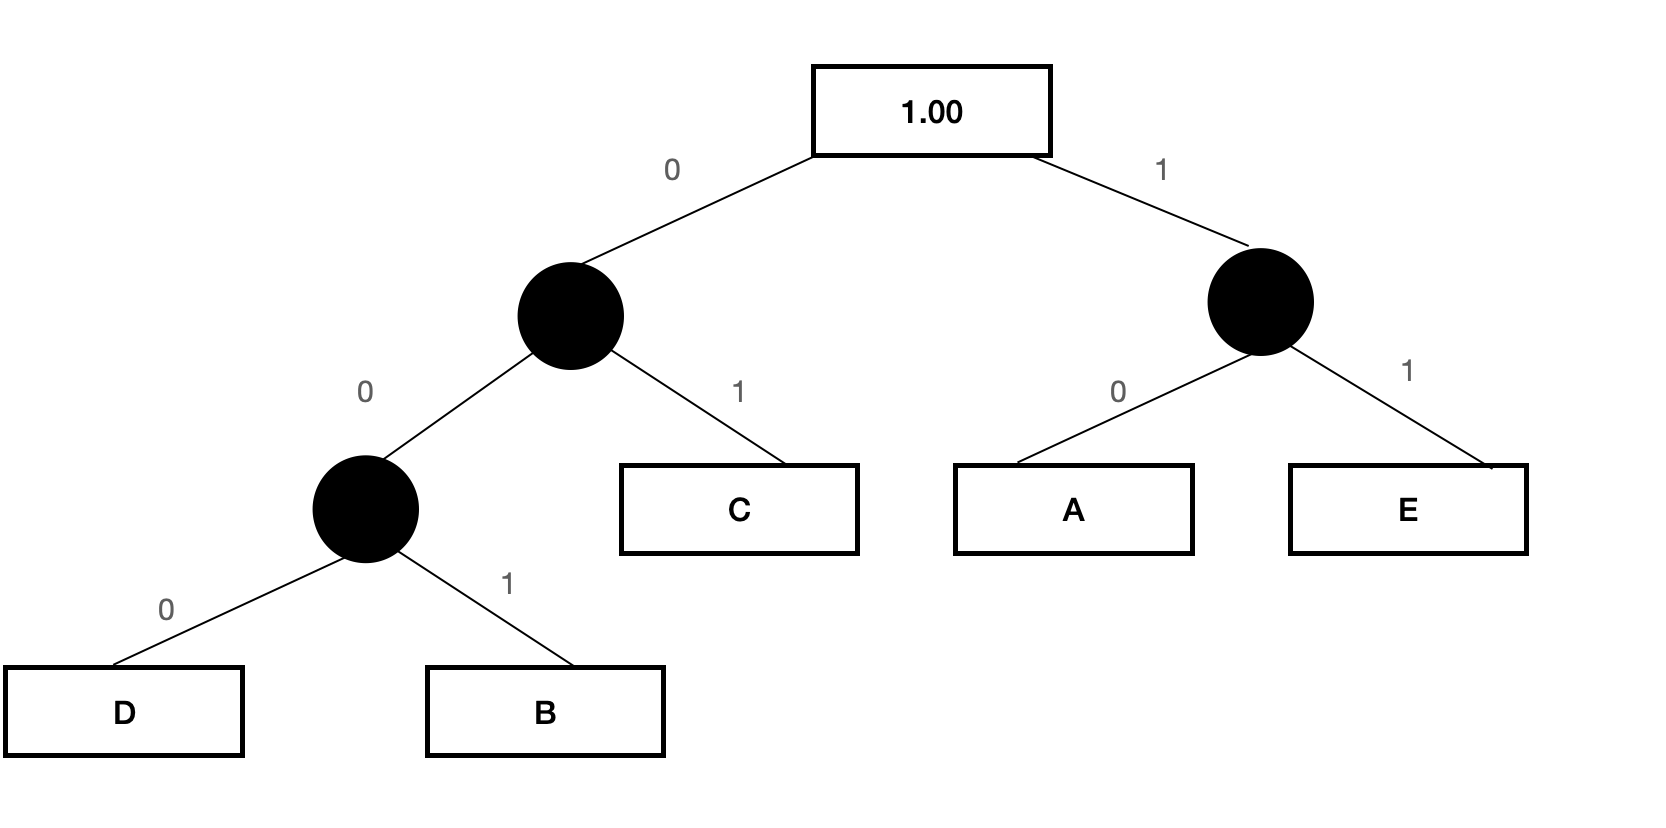
\includegraphics[scale=0.5]{tree}
    
\end{enumerate}

\fi

\newpage

%%%%%%%%%%%%%%%%%%%%%%%%%%%%%%%%%%%%%%%%%%%%%%%%%%%%%%%%
% PROBLEM FOUR %% PROBLEM FOUR %% PROBLEM FOUR %% PROBLEM FOUR %% PROBLEM FOUR %
%=======================================nb =======================================
% Problem 4: Basic Graph Search
%==============================================================================
% PROBLEM FOUR %% PROBLEM FOUR %% PROBLEM FOUR %% PROBLEM FOUR %% PROBLEM FOUR %
%%%%%%%%%%%%%%%%%%%%%%%%%%%%%%%%%%%%%%%%%%%%%%%%%%%%%%%%


\vspace{5mm}

\item The questions in this problem make use of the following weighted graph:

\begin{center}
	\begin{tikzpicture}[
	wide/.style={line width=4pt,arrows={-Stealth[length=15pt]}},
	node/.style={circle,draw,minimum size=16},
	directed/.style={arrows={-Stealth[length=8pt]}},
	scale=2]
	\node[node] (s) at (-0.5,0)            {$s$};
	\node[node] (u) at ($ (0,0) + ( 60:1)$) {$u$};
	\node[node] (v) at ($ (0,0) + (-60:1)$) {$v$};
	\node[node] (w) at ($ (u) + ( 1.5,0 )$) {$w$};
	\node[node] (x) at ($ (v) + ( 1.5,0 )$) {$x$};
	\node[node] (t) at ($ (w) + (-60:1) + (0.5,0)$) {$t$};
	\draw (s) to["8"] (u);
	\draw (u) to["5"] (w);
	\draw (s) to["1"] (v);
	\draw (v) to["9"] (x);
	\draw (u) to["7"] (v);
	\draw (x) to["2"] (w);
	\draw (w) to["3"] (t);
	\draw (x) to["4"] (t);
	\end{tikzpicture}
\end{center}

\begin{enumerate}
    \item List all simple paths from $s$ to $w$, along with their associated costs. (Note: A simple path is a path with no repeated vertices)
    
    To refer to a path, list the vertices in order in which they are encountered; for example, if you wanted to list the path from $s$ to $t$ along the top of the graph, you would write $(suwt, 16)$.
    
    \item Consider a form of depth first search that uses a greedy heuristic to decide which edge to traverse next from a given node. Once a node is selected for expansion, this approach orders the edges from that node by minimum cost. You can also assume this implementation of depth first search remembers previously-visited nodes and does not select edges that would visit them again. Starting from node $s$, what is the first path found from $s$ to $t$ and what is its cost? Is this the optimal path from $s$ to $t$? If not, give the optimal path.
    
    \item Using the version of depth first search described in (b), list the order in which depth first search visits all of the nodes if we start the algorithm from $u$.
    
\end{enumerate}

\if\solutions1
\vspace{3mm}
{\bf Solution}: \\
%==============================================================================
% STUDENTS: TYPE YOUR SOLUTIONS HERE. (Between \textbf{Solution:} and \fi )
%==============================================================================

\begin{enumerate}
    \item
        $(suw,13) \phantom{......} (svxtw,17) \phantom{......} (svxw,12) \phantom{......} (suvxw,26) \phantom{......} (suvxtw,31) \phantom{......} (svuw,13)$
    \item
        Using the DFS approach, the path from $s$ to $t$ would be: \\
        $$(svuwxt,19)$$\\
        The above path is optimal if all nodes must be visited
    \item
        Starting from $u$ the path would be: \\
         $$(uwxt,11)$$\\
         Since DFS are seeking the least cost between nodes, the above path would be the best choice for the given scenario.
\end{enumerate}

\fi


%========================================================================================================================

\een 


\end{document}